\section{Motivation} \label{sec:motivation}

%This section motivates for a more powerful function-merging technique with
%examples that highlight some of the weaknesses of the existing solutions, while
%also demonstrating how our optimization is able to overcome them.
%These examples contain real functions, extracted from the SPEC CPU2006 benchmark
%suite, that were carefully selected to show two distinct scenarios.
%The proposed optimization is the \textit{first} technique able to merge the
%functions shown in these examples.
%Note that, although we present the examples at the source level, the
%optimizations are actually implemented at the IR level.

As a motivation example, consider Figure~\ref{fig:sphinx-example} which shows to functions from the SPEC CPU2006 \texttt{482.sphinx3}
benchmark. Although these two functions seem identical, their function arguments are of different types, namely, \textit{float32} and
\textit{float64}. Here, we highlight the segments where the data operation differ from each other. As we have described in
Section~\ref{sec:background}, all the existing function-merging techniques require that both functions have exactly the same list of
parameters, with the same types and the same order. Moreover, this also means that the two functions contain instructions with different
types. As a result, no one of the existing techniques would be able to merge these two nearly identical functions.
However, these functions could be merged, as show at the bottom of Figure~\ref{fig:sphinx-example}.
First, we could merge the list of parameters, where we include the two parameters of different types.
Then, an extra parameter could be used as a function identifier to guard the execution of the instructions that
are unique to one of the functions.
If we inspect the compiled assembly code of all three functions, we can see a reduction of 18\% in the total number of machine instructions.
%If we compile all three functions, we can see that the each one of the two original functions have 14 machine instructions, while the merged function has 23 machine instructions.
%This represents a reduction of 18\% in the total number of instructions.
%However, the proposed optimization is able to merge them as shown at the bottom of Figure~\ref{fig:sphinx-example}. First, we merge both lists of parameters,
%adding an extra parameter used as an identifier to distinguish between the functions. Then, we guard the execution of the instructions that
%are unique to one of the functions using the function identifier. \fixme{ZW: Perhaps not talking about our technique here, but how much
%code reduction we can have by merging these two functions. We then use this to motivate the need of our technique.}

\begin{figure}[t!]
  \centering
  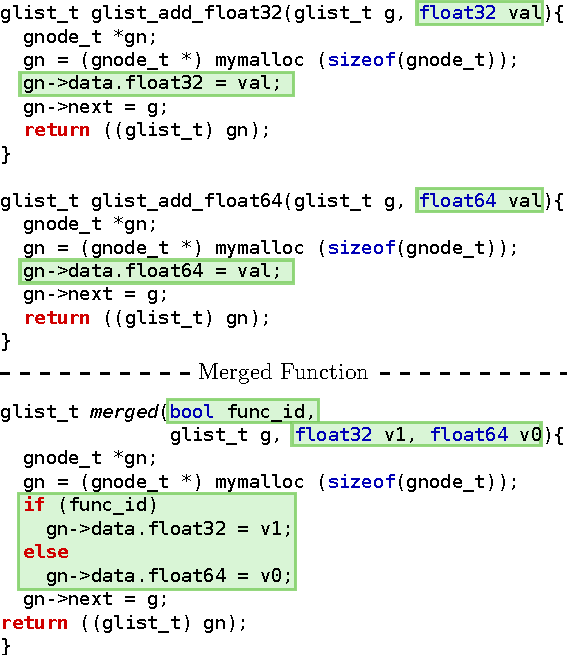
\includegraphics[width=.95\linewidth]{figs/sphinx-example.pdf}
  \caption{Functions with different list of parameters.}
  \label{fig:sphinx-example}
\end{figure}


Figure~\ref{fig:libquantum-example} shows two complete functions extracted from the SPEC CPU2006 \texttt{462.libquantum} benchmark.
Although these two functions have the same signature, i.e., the same return type and list of parameters, they differ in some parts,
including their CFGs. The existing techniques are unable to merge them due mainly to the structural differences in their CFGs, as we have
described in Section~\ref{sec:background}.
Similar to the previous example, we could merge these two functions, as shown at the bottom of Figure~\ref{fig:libquantum-example}. Basically, we just need to guard the execution of the code that are unique to
one of the functions using the function identifier added to the list of parameters.
Inspecting the compiled assembly of all three functions, we can see a reduction of 27\% in the total number of machine instructions.
%Similar to the previous example, the proposed optimization is also able to merge these two
%functions, as shown at the bottom of Figure~\ref{fig:libquantum-example}. Basically, we guard the execution of the code that are unique to
%one of the functions using the function identifier added to the list of parameters. \fixme{ZW: Again, here we need to give the intuition on
%why we can merge them and what's the benefit for doing so. I think we should avoid talking about our technique here because at this point
%the reviewer won't understand how our technique works.} 

\begin{figure}[t!]
  \centering
  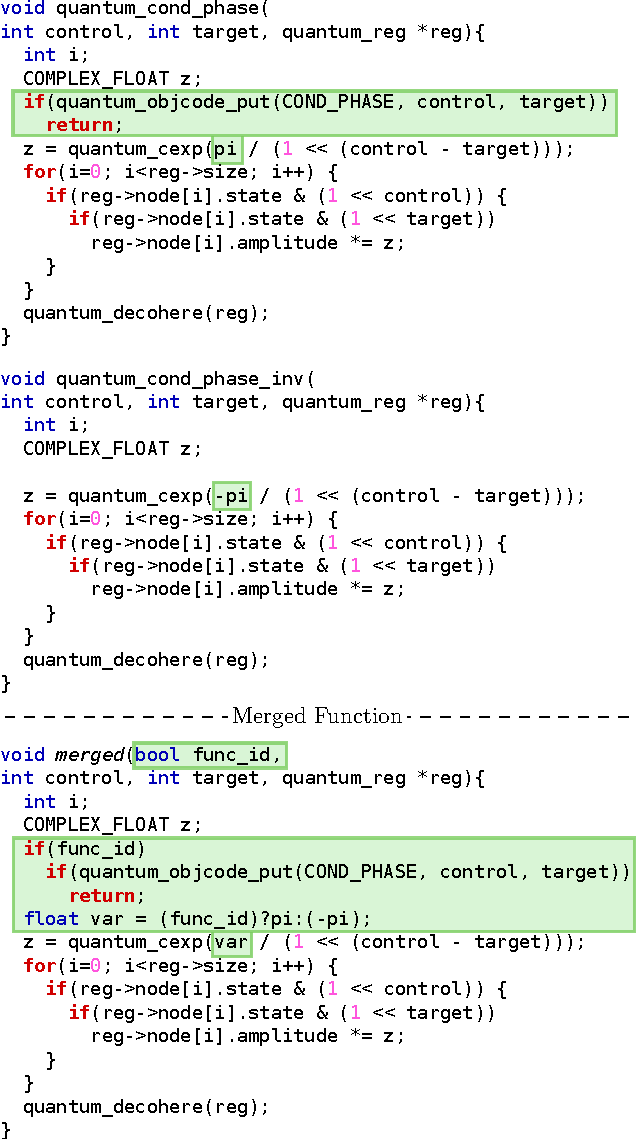
\includegraphics[width=\linewidth]{figs/libquantum-example.pdf}
  \caption{Functions with different CFGs.}
  \label{fig:libquantum-example}
\end{figure}
